\documentclass[conference]{IEEEtran}
\IEEEoverridecommandlockouts
% The preceding line is only needed to identify funding in the first footnote. If that is unneeded, please comment it out.
\usepackage{cite}
\usepackage{amsmath,amssymb,amsfonts}
\usepackage{algorithmic}
\usepackage{algorithm}
\usepackage{graphicx}
\usepackage{textcomp}
\usepackage{courier}
\usepackage{xcolor}
\def\BibTeX{{\rm B\kern-.05em{\sc i\kern-.025em b}\kern-.08em
    T\kern-.1667em\lower.7ex\hbox{E}\kern-.125emX}}
\begin{document}

\title{Improving Join Reordering for Large Scale Distributed Computing\\
}

\author{\IEEEauthorblockN{Amogh Margoor}
\IEEEauthorblockA{\textit{Qubole Inc.} \\
Santa Clara, US}
\and
\IEEEauthorblockN{ Mayur Bhosale}
\IEEEauthorblockA{\textit{Qubole Inc.} \\
Bangalore, India}
}

\maketitle

\begin{abstract}
SQL Join is one of the most commonly used operators for workloads running upon SQL Engines built for Big Data like Apache Spark SQL, Apache Hive and Presto. As Joins on Big Data can be expensive, Join optimizations can significantly improve the efficiency and performance of it's workloads. In this work, we would address the problem of finding optimal order for SQL Joins, which is a well researched NP-Hard problem for traditional workloads. Traditional Cost Based Optimization in Query processing, including Join Reordering algorithms are not effective on Big Data due to lack of statistics. Statistics are mostly absent in Big Data as they are expensive to compute and needs frequent recompute due to velocity of data change. Hence, ensuring optimal order of Joins for Big Data is still largely a manual process done via trial and error.

We are proposing a novel greedy algorithm for Join Reordering which can work in the absence of statistics. Proposed technique is of linear complexity in terms of number of joins. We have observed that on TPC-DS benchmarks it can reorder 39 queries and improve query performance upto 51\%.
\end{abstract}

\begin{IEEEkeywords}
SQL on Big Data, Query Processing, Join Order, Data Management Systems
\end{IEEEkeywords}

\section{Introduction}
\label{sec:intro} 
Massive analytics on Big Data using Large Scale Data processing are increasingly being used for business decisions. SQL Engines like Apache Spark~\cite{b9}, Apache Hive~\cite{b10} and Presto have been built for Big Data to address these needs. Such Engines have adapted many traditional DBMS relational techniques in this paradigm, making SQL operators like Join quite popular and common for Big Data Processing. For instance, on Qubole Data Service we see around 4 million joins getting processed every month through Apache Spark. Hence, optimizing Joins can improve the efficiency and performance of such workloads significantly. Finding optimal order of Joins is a very important Join optimization that can be extremely beneficial and hence, a well studied NP-Hard problem in traditional DBMS world.

Like in traditional systems, SQL Engines on Big Data also have Cost-Based Optimizer that can find the optimal join order using Dynamic Programming based algorithms \cite{b1}. However, availability of the extensive statistics like column statistics~\cite{b11} are pre-requisite for these traditional approaches. For instance, Apache Spark or Presto's Join Ordering will not work without the column statistics. In general, such statistics are absent for Big Data workload rendering these techniques ineffective. The volume of Big Data runs in TBs and PBs nowadays, associated with high velocity of change. Under such circumstances  computing statistics and maintaining it for new data changes can be expensive for the Data Administrators, hence almost never present.

An alternative to Cost Based approach to figure out optimal Join Order would be Adaptive query processing~\cite{b12}. Adaptive query processing can use runtime feedback to change the query plan being executed for better performance and efficiency. So even if statistics are not available, if such framework can compute statistics during runtime, it can be used to find optimal Join Order.
Firstly, such sophisticated framework is not present in many of the existing SQL engines for Big Data. Only Apache Spark has introduced support for it currently.  Secondly, 
even on Apache Spark, Adaptive query processing  do not provide column level stats at runtime from it's Query Stage which can be used to perform Join Reordering. Ensuring such elaborate statistics during runtime and waiting for all the Table Scan to finish for such statistics before starting any join can be detrimental to the performance of the query.

We analyzed the customer workloads at Qubole and couple of patterns emerged:
\begin{enumerate}
\item Statistics: Statistics were absent for almost all of the workloads. But  during planning stage, on-the-fly table sizes are computed by Apache Spark and Apache Hive if table sizes are not present. It is computed by listing the files under the table to obtain file metadata (with size information) and adding up the sizes of the each file. This is needed for doing the split planning as well as to ensure when joining with small tables, Broadcast Joins ~\cite{b13} on Spark or Map-Side Joins ~\cite{b10} on Hive can be performed which would make Joins faster. This is an important optimization which we briefly describe in Section ~\ref{subsubsec:sparkjoin}. These table sizes computation on the fly are the reason why among 4 million joins processed per month by Apache Spark on Qubole Data Service, 44 \% of them are Broadcast Joins as shown in Table ~\ref{tab:stats}. So even though, column level stats are not available, the table sizes are available during query planning.
\item Fact-Dimension Join: Another important pattern that emerged was that most of the queries with joins either on Snowflake schema or Star Schema will have Fact to Dimension table joins. Lot of queries with multi-table joins have 1 or multiple Fact tables involved in Join with other smaller dimension tables. That is the reason we see lot of Broadcast Joins (almost 44 \% of Joins according to Table ~\ref{tab:stats}) in Big Data workloads i.e., lot of small tables being used on one side of the Join.
\end{enumerate}

Based on the patterns above, in this paper we are presenting our technique for Join ordering using Table Sizes computed on-the-fly. Using the above patterns we devised a greedy technique for Join Reordering. At high level it performs two main steps:
\begin{enumerate}
\item Identify Dominant Fact table in a query i.e., Fact table involved in more than half number of Joins in the query. 
\item Perform Reordering of the Filtered Dimension tables involved in join with the Dominant Fact Table.
\end{enumerate}

Apart from the fact that this technique can work in absence of Statistics, it is also executes in linear time i.e., linear to the number of Joins in the Query. It is simple enough to be implemented as an Optimizer rule for the popular SQL engines on Big Data.  

We have implemented this technique in Qubole's distribution of Apache Spark as a Catalyst Rule. We have found it to be effective both on Customer workloads and TPC-DS benchmarks~\cite{b14} in spite of being simple to implement and reason about. When evaluated on TPC-DS benchmark~\cite{b14}  at 100 scale, we saw 39 queries being Join reordered among 100 queries. Out of all reordered queries, we were able to see a performance improvement in 71.8\% queries and only a marginal degradation in 28.2\% queries.

In the following Section ~\ref{sec:background} we will give a background on Joins, Statistics and Adaptive Execution in Big Data. Then we will propose our technique and algorithm in Section~\ref{sec:jo}. We will also present experimental evaluation of the algorithm in Section~\ref{sec:exp-evaluation}. In the following Section ~\ref{sec:rel_work}, we will discuss the existing work done in academia for Join Reordering and their relevance to our problem statement.

\section{Background}\label{sec:background}

In this section, we will review the popular Join algorithms in SQL Engines for Big Data and how will Join Reordering benefit those algorithms. Following that we will discuss the challenges with the traditional approaches for Join Reordering currently used in Big Data paradigm.

\begin{table}[h]
\begin{center}
\begin{tabular}{ |c|c| }
 \hline \\
Joins Processed & 3.9 million \\ \hline \\
Most common Join Type & INNER JOIN - 51\%  \\  \hline \\
Second most common Join Type &  LEFT OUTER JOIN - 31\%\\ \hline  \\
Most common Join algorithm & SortMergeJoin - 55\%\\ \hline \\
Second most common Join algorithm & BroadcastHashJoin - 44\%\\
 \hline
\end{tabular}
\label{tab:stats}
\end{center}
\caption{Join metrics collected over 1 month for Apache Spark in Qubole}
\end{table}

\subsection{Why is Join Reordering important ?}
All the prominent SQL Engines for Big Data like Apache SparkSQL, Presto, Hive etc  have Cost Based Join Reordering which give them multiple Xs in performance improvement\cite{b2}.

Let's look closely into how it can affect a query performance. For illustration, we will pick commonly used Join Algorithm in Presto and Apache Spark. Hash Join is commonly used distributed join in Presto and Sort Merge Join in Apache Spark.

\subsubsection{Distributed Hash Joins in Presto}

\begin{figure}[ht]
\centerline{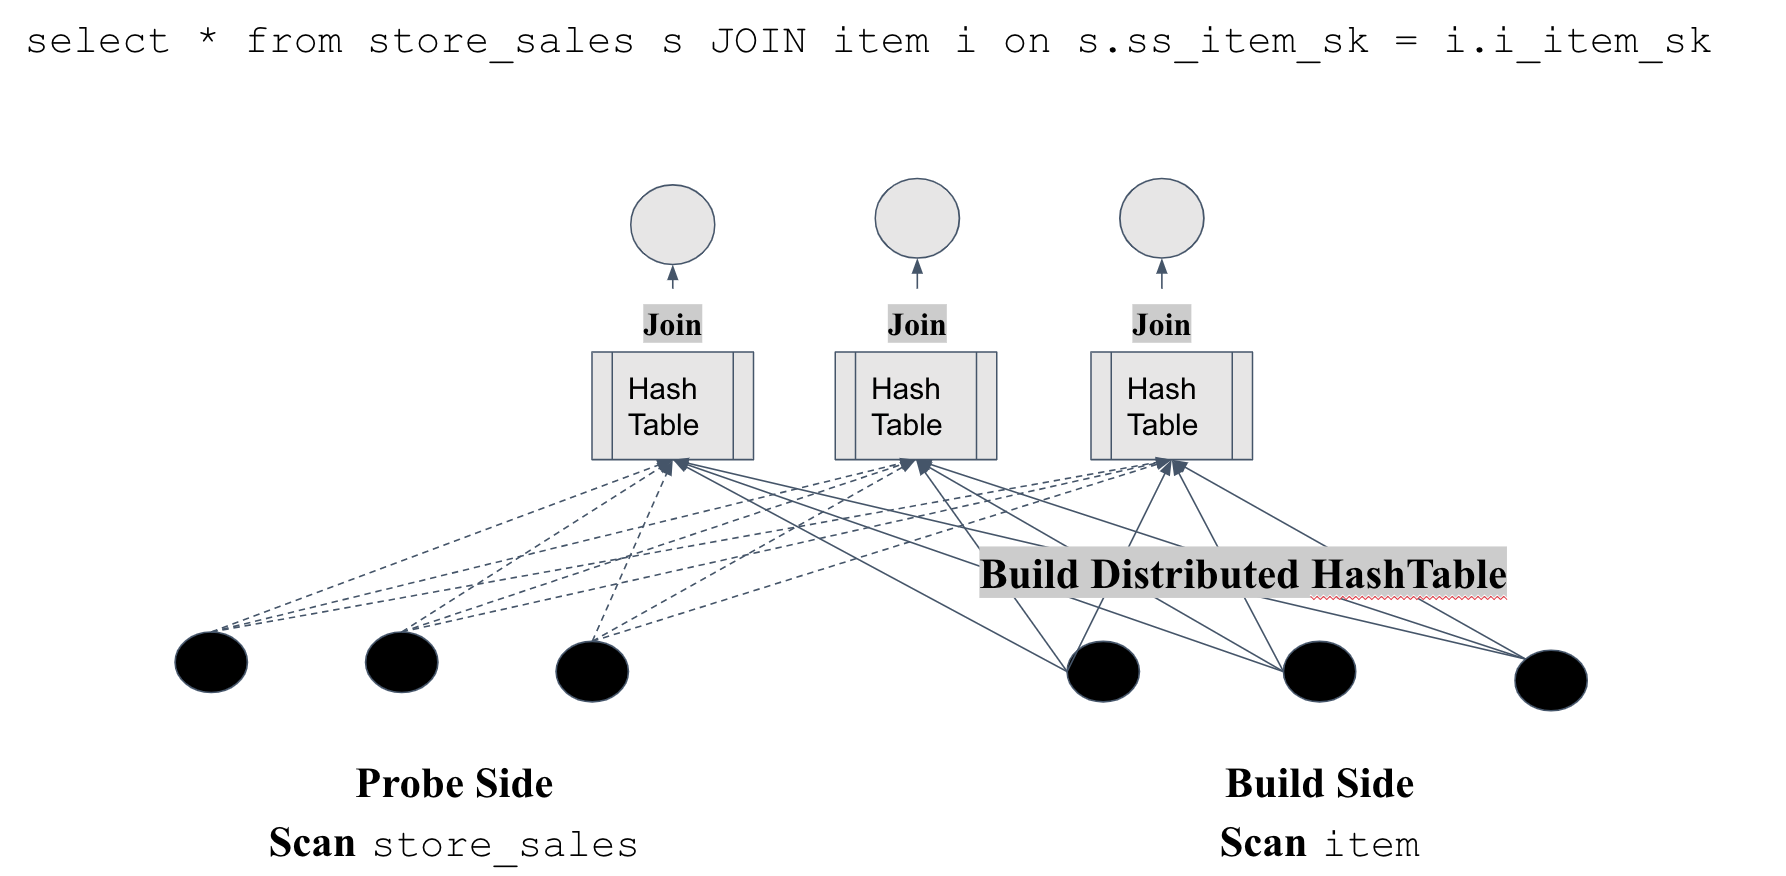
\includegraphics[width=9.5cm]{fig/DistributedHashJoin.png}}
\caption{Distributed Hash Join}
\label{distributed_hash_join}
\end{figure}

Hash Join is most commonly used distributed join algorithm in Presto.
Figure \ref{distributed_hash_join} illustrates this join.
When joining two tables \texttt{store\_sales} and \texttt{item} Presto regards table on the right i.e., \texttt{item}  as build side and table on left i.e., \texttt{store\_sales} as probe side.
Build side is used to build distributed hash table. As shown in the figure, after table \texttt{item} is scanned, its rows are hash distributed to different nodes based on join key \texttt{i\_item\_sk}. Once distributed, rows from table B are used to create Hash Table. Rows from the Probe Side are also distributed to different nodes using the same hash on the join key \texttt{i\_item\_sk}. Due to this partitioning \texttt{ss\_item\_sk}  and \texttt{i\_item\_sk} with same values end up in the same node.  Rows of Probe Side once distributed are checked against Hash table to find matching join rows. Here, major cost of the join will be building Hash tables on the Build Side. Hence, join reordering can considerably improve the performance by choosing smaller table as build side whenever possible (like in the cases of INNER Joins).

\subsubsection{Sort Merge Join in Spark}\label{subsubsec:sparkjoin}

\begin{figure}[ht]
\centerline{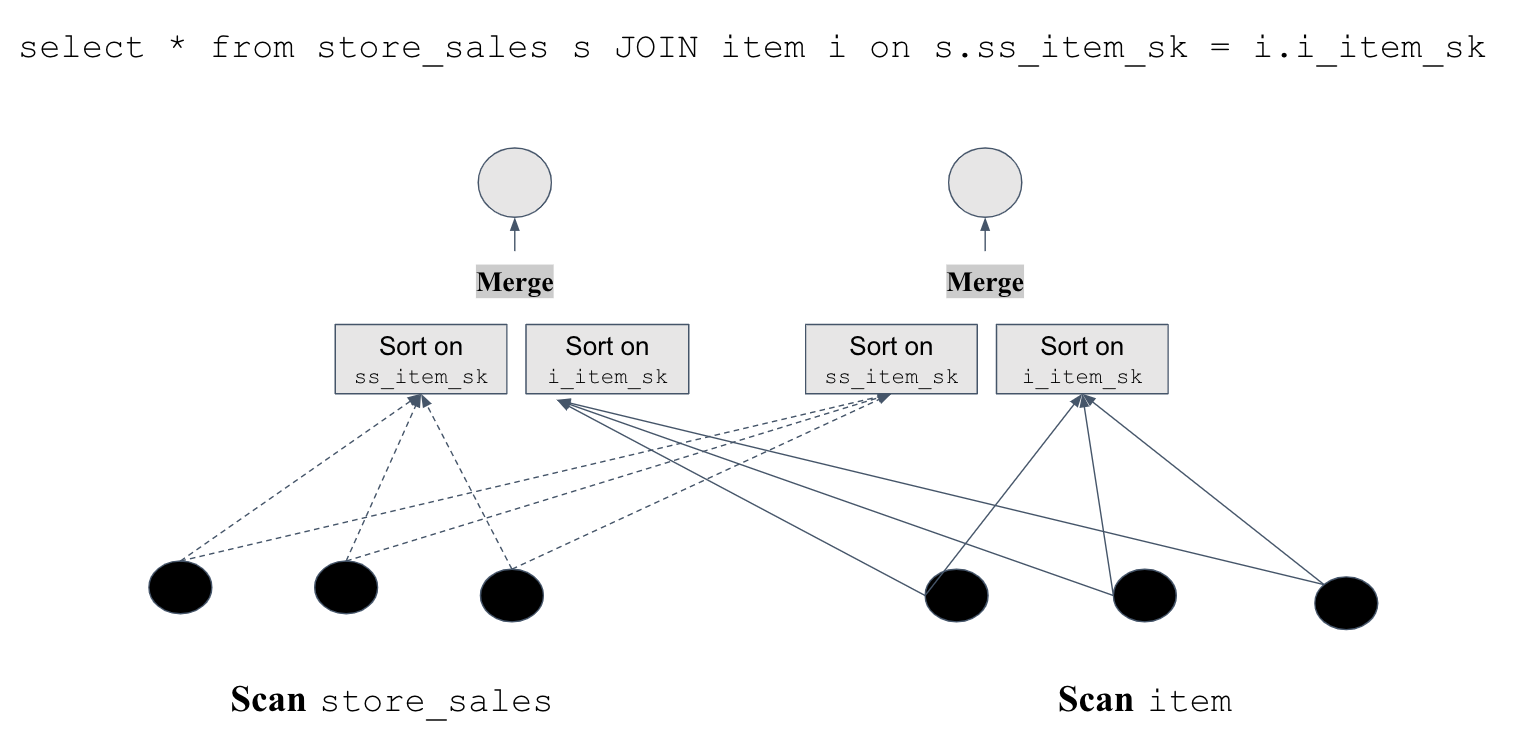
\includegraphics[width=9.5cm]{fig/SortMergeJoin.png}}
\caption{Sort Merge Join}
\label{sort_merge_join}
\end{figure}

Spark implements both Sort Merge Join and Hash Join.
Hash Joins are commonly used for Broadcast Joins, where if one of the sides of join is less in size than the threshold set by \texttt{$sql.autoBroadcastJoinThreshold$} then that side's hash table gets broadcasted to nodes with other larger side.
Join is performed locally on those nodes against the broadcasted hash table.

Except for the above case, Sort Merge Join is most commonly used join in Spark. Figure \ref{sort_merge_join} illustrates the Sort Merge Join.
Both tables \texttt{store\_sales} and \texttt{item} are distributed based on hash partitioning on join keys i.e., \texttt{ss\_item\_sk} and \texttt{i\_item\_sk} respectively. Due to this partitioning \texttt{ss\_item\_sk}  and \texttt{i\_item\_sk} with same values end up in the same node. Once rows from each table are distributed, they are individually sorted locally in every node and they are merged together to perform join. Internally Spark while doing merge uses scanner where for every key being considered for merging, one side will be streamed and another side will have rows with merge key buffered. Buffered rows can be spilled to disk too if it crosses memory threshold. In case of INNER Join, left side is streamed and right one will be buffered. So it is better to ensure the buffered side is the smaller one for lesser memory consumption and to avoid spill (spill can affect performance adversely). Hence, Join reordering is essential.

Both the above examples I provided were for a single join. In case of multi-way Join, reordering becomes even more important and can lead to huge performance improvements.
\subsection{Current State of Statistics and Join Reordering Algorithm for Big Data}

Currently, all these engines either use the Hive statistics or have statistics similar to it \cite{b1}:
\begin{itemize}
\item totalSize: Total size of the dataset as its seen at the filesystem level.
\item numFiles: Number of files the dataset consists of.
\item rawDataSize: Uncompressed size of the dataset.
\item numRows: Number of rows in the dataset.
\item columnStatistics: Statistics at column level: number of distinct values, max value, min value, number of null values, max length, average length.
\end{itemize}


In above, subsection we clearly saw why traditional approaches like Cost-Based Optimizations and Adaptive Execution not work well for finding optimal Join Order in Big Data. Hence, in this paper we will present a novel greedy approach for Join Reordering which can work without expensive statistics for Big Data Systems.

\section{Join Reordering without statistics}\label{sec:jo}
In the previous section we looked into the current state of affair for Join Reordering and why would it not work for Big Data systems. We will like to propose a novel approach in this section to reorder Join just based on the table sizes without any elaborate Table or Column Statistics as required by existing approaches.
We have implemented this approach in Apache Spark and will show how our approach gives up to X improvement in TPCDS queries in our empirical evaluation.

\subsection{Heuristics}

Let us look at the assumptions and heuristics used for the approach.

\subsubsection{Assumptions}\label{subsubsec:assumption}:

\begin{itemize}
\item In Star Schema Join, the Dimension table’s primary key will be joined with the Fact table’s foreign key.
\item Cardinality of Fact Table joined with Filtered Dimension table will be less than that of the Fact table.
\item So based on the last assumption, it follows that if Fact Join with Filtered Dimension happens earlier in multi-way join, it can benefit later joins.
\end{itemize}

To illustrate assumption above, let's look at this query:
\texttt{select * from fact\_table f join dim1 d1 on f.k1 = d1.pk join dim2 d2 on f.k2 = d2.pk where d2.date = ‘06-10-2019’}. If there is a filter on \texttt{dim2} which is smaller than \texttt{dim1} assumption is, it’s join with \texttt{fact\_table} would be smaller than \texttt{fact\_table}. Hence, joining \texttt{fact\_table} with \texttt{dim2} and then with \texttt{dim1} will be beneficial.

\subsubsection{Heuristics for detecting Star schema}
In the lack of relations information and statistics, we have to use only table sizes and query structure to determine if a Join is a start schema. We are using the following heuristics to determine them:

\begin{itemize}
\item Table involved in all of the joins should be a fact table.
\item At least half of the inner joins in the query should involve the fact table.
\item The ratio of the size of the largest dimensions table to fact table size should be lesser than a certain threshold.
\item None of the dimensions tables should be partitioned.
\end{itemize}

\subsubsection{Constraints for the Join Reorder algorithm}
We will define all the constraints or boundary conditions for the applicability of the algorithm here:

\begin{itemize}
\item \textbf{Star Schema Constraint}: Only Star schema Joins will be considered as assumptions made above are for Star Schema Join only.
\item \textbf{Simple Join Constraint}: Only INNER Joins whose left and right side are comprised of these operators that are deterministic and which do not increase the output size over the input size, other than Join.
\item \textbf{Shuffle Constraint}: For systems having shuffle like Spark or Hive, we reorder only if the number of shuffles do not increase due to it. For e.g., consider the following query: \texttt{select * from store\_sales s, item i, web\_sales ws, customer c where s.ss\_item\_sk = i.i\_item\_sk and i.i\_item\_sk = ws.i\_item\_sk and c.c\_customer\_sk = s.ss\_customer\_sk}
\item \textbf{Size Constraint}: Fact table should be at least $X$ times larger than dimension tables. $X$ is configurable.
\end{itemize}

\subsection{Algorithm}

\begin{algorithm}
\begin{algorithmic}[1]
\STATE  $\Omega$ $\gets$ $R_1$ $\Join$ $R_2$
\IF{$isStarSchemaJoin$($\Omega$) and $isSimpleJoin$($\Omega$) and $obeysShuffleConstraint$($\Omega$)}
    \STATE $type$ $\gets$ $treeType$($\Omega$) \COMMENT{$type$ will be either $left-deep$ or $right-deep$}
    \STATE ($\sigma$, $\delta$[$1$, $\ldots$, $n$]) $\gets$ $extractFactDimensions$($\Omega$)
    \STATE $\theta$[1, $\ldots$, k] $\gets$ $getFilteredDimensions$($\delta$[$1$, $\ldots$, $n$])
    \STATE $\pi$[1, $\ldots$, l] $\gets$ ($\delta$[$1$, $\ldots$, $n$] - $\theta$[1, $\ldots$, k]
    \STATE $\theta$[k+1] $\gets$ $dummyTable1$
    \STATE $dummyDim1$.$size$ $\gets$ $\infty$
    \STATE $\pi$[l+1] $\gets$ $dummyTable2$
    \STATE $dummyTable2$.$size$ $\gets$ $-\infty$
    \STATE $i$ $\gets$ 0
    \STATE $j$ $\gets$ 0
    \FOR{$r$ $\gets$ $1$ to $n$}
        \IF{$\theta$[$i$].size $\geq$ $\pi$[$j$].size}
            \STATE $i$ $\gets$ $i$ $+$ $1$
            \STATE $result$[$r$] $\gets$ $\theta$[$i$]
        \ELSE
            \STATE $j$ $\gets$ $j$ $+$ $1$
            \STATE $result$[$r$] $\gets$ $\pi$[$j$]
        \ENDIF
    \ENDFOR
    \STATE $\Omega$ $\gets$ $buildJoinTree$($type$, $\sigma$, $result$[$1$, $\ldots$, $n$])
\ENDIF
\RETURN $\Omega$
\end{algorithmic}
\label{algorithm}
\caption{Algorithm to Reorder Joins}
\end{algorithm}


In the algorithm presented above, $\Omega$ is assigned to the input Join that needs to be reordered. Following are the summary of steps to reorder them:
\begin{itemize}
\item Check if all constraints are satisfied for a join: \textbf{Star Schema Constraint}, \textbf{Simple Join Constraint}, \textbf{Shuffle Constraint}, \textbf{Size Constraint}.
\item Once it is a star schema, the Join tree can either be \textit{left-deep} or \textit{right-deep}. Obtain the information as we would like to construct reordered join the same way.
\item Extract the Fact table: $\sigma$ and Dimension tables: $ (\delta_1, \delta_2, \ldots, \delta_n)$. For dimension table, $\delta_i$ represents  $i^{th}$ dimension table being joined with the fact table $\sigma$ from the bottom of the Join Tree as shown in Figure \ref{left-deep}. As the tree here would be either \textit{left-deep} or \textit{right-deep} every dimension will have unique $i$ assigned to them.
\item Split dimensions into two lists: one with selective predicates. $\theta$ and another without it, $\pi$.
\item Sort the list with selective predicates i.e., $\theta$ based on sizes of the dimension tables. Sort the other list i.e., $\pi$ using user-provided order.
\item Merge both the list of dimensions by giving user order the preference for tables without a selective predicate, whereas for tables with selective predicates giving preference to smaller tables. When comparing the top of both the lists, if size of the top table in the selective predicate list is smaller than top of the other list, choose it otherwise vice-versa. This is in congruence with the Assumption made earlier in subsection \ref{subsubsec:assumption}.
\end{itemize}

\begin{figure}[ht]
\centerline{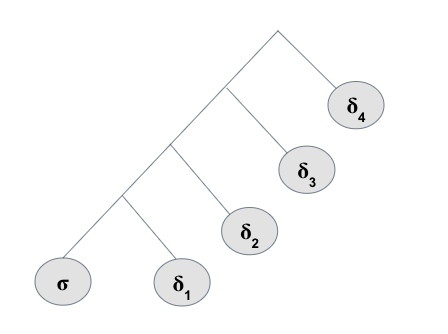
\includegraphics[width=5cm]{fig/left-deep.png}}
\caption{Left-Deep Tree with Fact table $\sigma$ and dimension tables $\delta_i$}
\label{left-deep}
\end{figure}


We evaluated the above mentioned greedy heuristics based approach in a Apache Spark. Spark's SQL optimizer allows passing the optimizer rules externally to the application. We implemented an optimizer which takes the optimized plan as input and based on the heuristics proposed, reorders the joins wherever applicable . It is assumed that the table sizes are available in the Spark optimized plan before applying this rule. We used the TPC DS dataset (scale 1000) non-partitioned dataset for evaluating the performance. The experiments was ran on a 5 node Apache Spark cluster on AWS with machine type r4.4xlarge.

Out of 100 TPC-DS queries, we were able to reorder at least one join in the 41 queries. For the queries not reordered, the performance would be same as before. Figure 4 shows the runtime of few of the queries with and without the optimisation. We saw approximately 28\% improvement in the reordered queries and no performance degradation in any of the reordered query.

\begin{figure}[ht]
\centerline{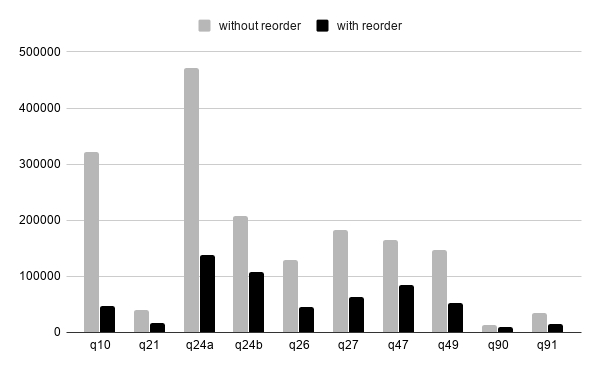
\includegraphics[width=7cm]{fig/chart.png}}
\caption{Performance reordered sample queries}
\label{performance_number}
\end{figure}
\section{Related Work}\label{sec:rel_work}
A lot of work has happened in the domain of the query planning of which the join ordering and join strategy are key components. It is agreed upon that the join reordering problem, in particular, is NP-Hard. There are quite a few approximation algorithms that try to solve this problem by leveraging the fact that not all join combinations are valid. System R \cite{b1} first suggested the use of Dynamic Programming (DP) for join ordering and is widely used by the join optimizers. DP based approach like System R come up with all possible valid join combinations and then chooses the plan with minimum cost. Guido and Thomas \cite{b3} propose a more optimised graph based dynamic programming strategy by avoiding the combinations which will not lead to valid join trees. The cost function for estimating the cost of running a given plan for both the approach relies heavily on column level statistics like cardinalities, and distinct values for defining the cost function.

The DP based approaches are not scalable as they have exponential run time as well as space complexity. So these techniques are only feasible when the number of joins is small. Spark for example, only reorders joins involving less than 12 relations. Large ad-hoc queries involving more than 10 relations are common in modern-day online analytical processing (OLTP) and object-oriented databases as the SQL queries are often nested. To tackle this problem,  the literature described in [\cite{b4}, \cite{b5}, \cite{b6}] proposes a heuristics-based approach for finding the optimal join order. These systems build the joins greedily either from a bottom-up or a top-down manner.  Heuristics based approaches are different compared to the DP based approaches that, rather than minimizing the cost of the entire plan they try to minimize the cost at each step. All though, greedy based approaches may not always produce the most optimal order, the primary goal here is to find a more optimal order compared to the current order.

Both DP and Greedy approached rely on the column level statistics like cardinalities and distinct values. Generating and maintaining these statistics require a full table scan making it infeasible to maintain stats especially in frequent write scenarios. [Insert number of cases where stats are not available]. Even if the statistics are available, operators between the scan of the table and join can alter the data making the statistics inaccurate. Adaptive query execution removes the hard dependency of collecting the up-front statistics and the assumption of their accuracy by reordering the query plan on the fly rather than doing it at the start. In batched query systems like Spark, adaptive collects the statistics after executing all substage below the shuffle boundary.
The newly generated statistics are then used for query replanning on the fly. This procedure is recursively applied at each shuffle boundary to leverage the newly updated statistics. Literature \cite{b7} proposes reordering of the plans containing the nested loop joins after executing every batch of rows from the driver table based on the match rate of the joins. This approach however does not work for other join types because all the tables scans start in parallel. The  RIOS \cite{b8} takes a blocking approach where it starts by executing the pre-shuffle stages and then samples the data thus generated to get the information on cardinality and unique keys. Even though this approach is generic for all join types, the overhead of the sampling the data at shuffle stages and making blocking execution makes this approach infeasible in production environments. [Add numbers]

\section{Conclusion and Future Work}
We discussed the commonly used Join algorithm in Big Data Engines and benefits of Join Reordering for them. Then we looked into how traditional approaches fail in Big Data paradigm. This motivated us to propose a novel algorithm that can be used in Big Data Engines where statistics are scarce. We evaluated this technique on widely popular TPC-DS benchmark to observe it's benefit. The focus of the work was to study the benefits of a simpler technique in scenario where more sophisticated techniques failed in Big Data paradigm. As a future work:

\begin{itemize}
\item Continue to identify and handle more query patterns for Reordering.
\item Eliminate regressions of any kind due to this.
\item Integrate this approach more tightly with Adaptive Execution to atleast obtain more accurate sizes of the plan.
\end{itemize}



\begin{thebibliography}{00}
\bibitem{b1} Selinger, P. Griffiths, M. M., Astrahan, D. D., Chamberlin, R. A., Lorie, and T. G., Price. ``Access Path Selection in a Relational Database Management System.`` . In Proceedings of the 1979 ACM SIGMOD International Conference on Management of Data (pp. 23–34). Association for Computing Machinery, 1979.
\bibitem{b2} Amogh Margoor, Rajat Venkatesh. ``SQL Join Optimizations in Qubole Presto,``
https://medium.com/qubole-engineering/sql-join-optimizations-in-qubole-presto-3ced3dc75275, unpublished
\bibitem{b3} Guido Moerkotte and Thomas Neumann. 2006. ``Analysis of Two Existing and One New Dynamic Programming Algorithm for the Generation of Optimal Bushy Join Trees without Cross Products.`` In Proceedings of the 32nd International Conference on Very Large Data Bases, Seoul, Korea, September 12-15, 2006. 930–941.
\bibitem{b4} A. Swami ``Optimization of large join queries: combining heuristics and
combinatorial techniques.`` SIGMOD Record, vol. 18, no. 2, 1989.
\bibitem{b5} L. Fegaras ``A new heuristic for optimizing large queries in DEXA ’98``. Proceedings of the 9th International Conference on Database and Expert Systems Applications, 1998.
\bibitem{b6} N. Bruno, C. Galindo-Legaria and M. Joshi ``Polynomial Heuristics for Query Optimization``. 2010 IEEE 26th International Conference on Data Engineering (ICDE 2010), Long Beach, CA, 2010, pp. 589-600, doi: 10.1109/ICDE.2010.5447916.
\bibitem{b7} Li, Quanzhong and Shao, Minglong and Markl, Volker and Beyer, Kevin and Colby, Latha and Lohman, Guy. (2007)  ``Polynomial heuristics for query optimization,`` Proceedings - International Conference on Data Engineering. 26-35. 10.1109/ICDE.2007.367848.
\bibitem{b8} Li, Youfu and Li, Mingda and Ding, Ling and Interlandi, Matteo. (2018)  `` RIOS: Runtime Integrated Optimizer for Spark`` 275-287. 10.1145/3267809.3267814.
\bibitem{b9} M. Zaharia, M. Chowdhury, M.J. Franklin, S. Shenker, I. Stoica
``Spark: Cluster computing with working sets`` Proceedings of the 2Nd USENIX Conference on Hot Topics in Cloud Computing, HotCloud’10, USENIX Association, Berkeley, CA, USA (2010), p. 10 http://dl.acm.org/citation.cfm?id=1863103.1863113
\bibitem{b10} Apache Hive. http://hadoop.apache.org/hive.
\bibitem{b11} The Internals of Spark SQL. https://jaceklaskowski.gitbooks.io/mastering-spark-sql/content/spark-sql-ColumnStat.html
\bibitem{b12} Avnur R. and Hellerstein J.M. Eddies: ``continuously adaptive query processing.`` In Proc. ACM SIGMOD Int. Conf. on Management of Data, pp. 261–272.2000
\bibitem{b13} Armbrust, M., Reynold Xin, Cheng Lian, Yin Huai, Davies Liu, Joseph K. Bradley, X. Meng, Tomer Kaftan, M. Franklin, A. Ghodsi and M. Zaharia. ``Spark SQL: Relational Data Processing in Spark.`` SIGMOD '15 (2015)
\bibitem{b14} Meikel Poess, Bryan Smith, Lubor Kollar, and Paul Larson. 2002. ``TPC-DS, taking decision support benchmarking to the next level.``  In Proceedings of the 2002 ACM SIGMOD international conference on Management of data (SIGMOD '02). Association for Computing Machinery, New York, NY, USA, 582–587. DOI:https://doi.org/10.1145/564691.564759
\end{thebibliography}
\end{document}
